\section{Experiments and Results}
\label{sec:results}
% Furkan
% LLM experiments

% \begin{figure*}[h!]
% \includegraphics[width=\textwidth]{figures/ImpactOfUDReval.eps}
% \caption{\label{fig:impactoffeatureadditionandremoval} The impact of the addition and removal of features on the accuracy.}
% \end{figure*}

\begin{figure*}
    \begin{subfigure}{\textwidth} % 50% of the text width
        \centering
        \fbox{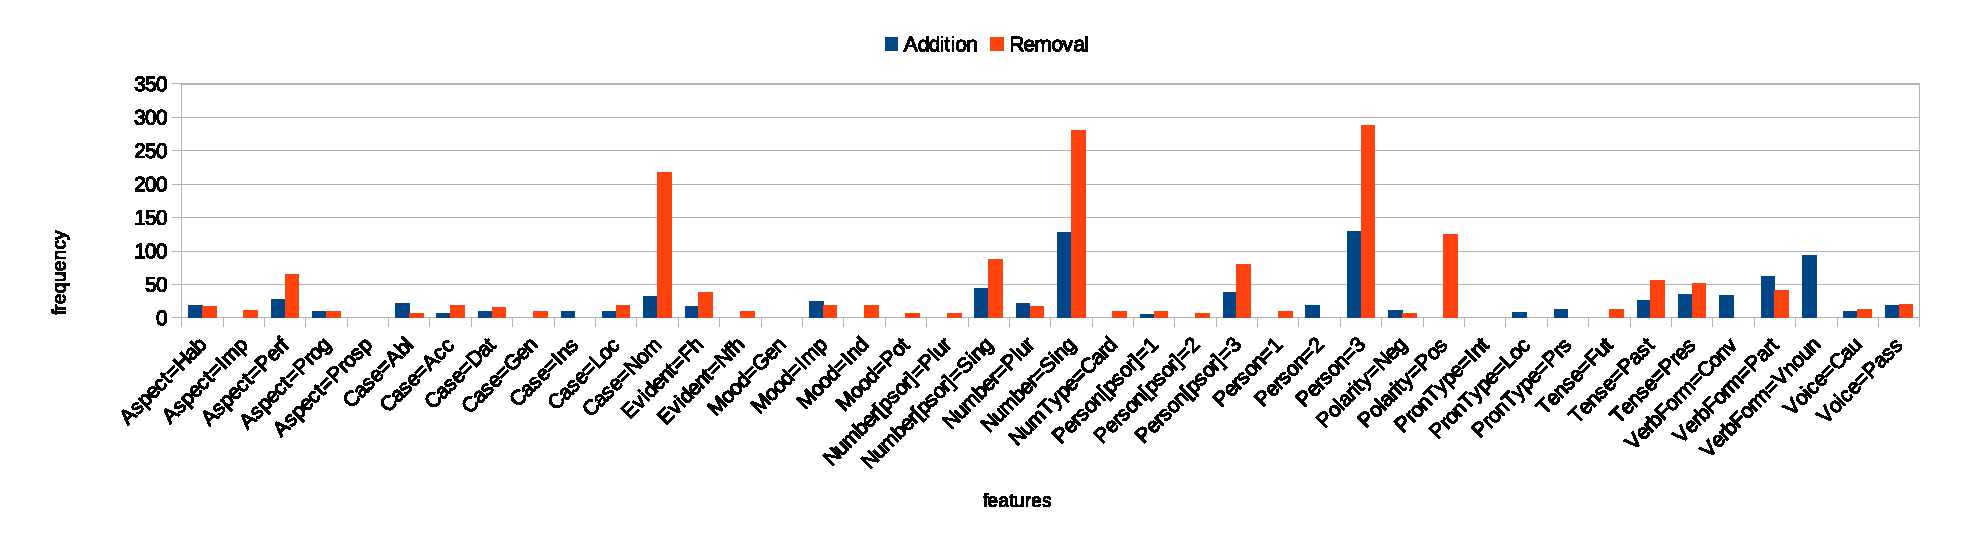
\includegraphics[width=0.99\linewidth]{figures/performance-incrase.eps}}
        \caption{The addition or removal of the features that improved the recovery.}
        \label{fig:subfig1}
    \end{subfigure}%
    
    \begin{subfigure}{0.9\textwidth}
        \centering
        \fbox{\includegraphics[width=1.1\linewidth]{figures/performance-decrease.eps}}
        \caption{The addition or removal of the features that reduced the recovery.}
        \label{fig:subfig2}
    \end{subfigure}
    \caption{\label{fig:impactoffeatureadditionandremoval} The impact of the addition and removal of features on the accuracy. }
\end{figure*}

\begin{table}
\centering
\begin{tabular}{|l|c|c|}
\hline
\multicolumn{1}{{|c|}}{\textbf{Model}} & \multicolumn{1}{{c|}}{\textbf{v2.8}} & \multicolumn{1}{{c|}}{\textbf{v2.11}} \\ \hline
GPT-3.5-Turbo       & 83.58          & 84.52    \\ \hline
Claude-instant-100k & 85.95          & 87.36    \\ \hline
GPT-4               & 89.97          & 91.28    \\ \hline
Claude-2-100k       & 89.00          & 90.53    \\ \hline
\hline 
& \multicolumn{2}{c|}{\textbf{UD\_English-EWT}}  \\ \hline
GPT-4              & \multicolumn{2}{c|}{94.00}  \\ \hline
\end{tabular}
\caption{The accuracy by sequence matching scores of the experiments with various large language models provided for \bounvOLD\ and \bounvNEW. The result for \ewt\ is provided for reference.}
\label{tab:results}
\end{table}


Several experiments using different large language models were conducted to compare alternative annotations of the same treebank. 
Specifically, the GPT-3.5, GPT-4~\cite{openai}, Claude Instant, and Claude 2~\cite{claude} models were prompted using the Poe API~\cite{poe}.

The proposed method was implemented with 500 randomly selected sentences that are consistent with the distribution of the number of tokens per sentence in the treebanks. 
A prompt was generated  for each annotated version of these sentences as explained in Section~\ref{sec:method}.
API calls were made to the above-mentioned models with these prompts and their responses were processed. 
Table~\ref{tab:results} shows the accuracy by sequence matching for both models.
Across all experiments, we observe a consistent increase of approximately 1.5\% in accuracy for \bounvNEW. 
This suggests that its annotations better capture the features of the sentences.

We also experimented with a treebank of another language, the \ewt\ treebank, to validate the method.
As GPT-4 produced the best results, we used only this model for this experiment.
The table shows that the model yields better recovery than all the models used for Turkish.
This may be regarded as an expected result since the GPT-4 model better captures the English language, and English sentences are somewhat easier to recover as they do not possess complex morphological features such as    morphologically rich languages like Turkish do.

Figure~\ref{fig:impactoffeatureadditionandremoval} illustrates the impact of adding and removing features during the re-annotation phase.
The most substantial improvement, attributed to the unique morphological feature tag and value, was achieved by removing the third-person annotation (i.e., Person=3) from a single token in the treebank during the transition from v2.8 to v2.11.
This change aided in producing the correct token 288 times, while it also led to the model producing an incorrect token 189 times.
The fact that the same feature tag and value pair (the third-person annotation) resulted  in both the most significant improvement and worsening of the performance underscores its significance in token recovery.
In Turkish, the third person is represented by two exponents: a null morpheme for singular and \textit{-lAr} for plural.
The fact that, as discussed in the previous sections, addressing a significant issue in Turkish that the UD framework has overlooked has had a notable impact on token recovery underscores the necessity to reconsider certain preconceptions and assumptions made by the UD framework regarding null morphemes.

While the removal of case and number can reduce accuracy in certain instances, it generally enhances overall performance. This suggests that the v2.8 version of the treebank may have had some level of clutter. Furthermore, the consistent improvement in annotation precision is observed when new features are added. It is essential to note that the addition of new features should be undertaken judiciously to prevent clutter and the annotation of non-existing layers of meaning.

To gain insight into the impact of annotations on recovering the surface forms of the sentences, various failures have been examined.
The reported accuracy scores are based on sequence matching over the entire sentence.
To gain a better understanding of the parts of the sentences that were not recovered accurately, the words within the sentences are examined along with their annotations.
By doing so, we aimed to understand the impact of the annotations in this task.
Since Turkish is a morphologically rich agglutinative language, the recoveries of the suffixes and their ordering are highly significant.

The percentage of produced tokens that matched the tokens and their order in the original sentences via prompting the GPT-4 model with the annotations from \bounvOLD\ and v2.11 are 73.7\%  and 75.4\% respectively (total number of tokens is \num{6247}).
The frequencies of the top five features for the words that were not  accurately recovered are shown in Table~\ref{tab:word-error-feature-analysis}. 

Except for polarity, these features belong to the nominal domain of Turkish, which is characterized by a high degree of syncretism. For example, the third-person possessive marker, \textit{-ı}, shares the same form as the accusative marker, \textit{-ı}. Consequently, this is an area where language models or parsers not engaged in syntax may struggle, as seen in v2.8. However, this confusion appears to have been minimized in v2.11. 

Additionally, the impact of  modifying the values of features was examined.
Table~\ref{tab:featurechange} shows the frequencies of improvement and worsening recovery for the most frequently used feature tags.

\begin{table}[tbh!]
\centering
\begin{tabular}{|l|S[table-format=4] | l | S[table-format=4] | l|}
\hline
\multicolumn{1}{|c|}{\textbf{Feature}} & \multicolumn{2}{c|}{\textbf{v2.8}} &  \multicolumn{2}{c|}{\textbf{v2.11}} \\ \cline{2-5} 
 & \multicolumn{1}{c|}{\textbf{\#}} & \multicolumn{1}{c|}{\textbf{\%}} & \multicolumn{1}{c|}{\textbf{\#}} & \multicolumn{1}{c|}{\textbf{\%}} \\ \hline
Person=3 & 1185 & 37 & 1167 &  35 \\ \hline
Number=Sing & 1072 & 36 & 1054 & 35 \\ \hline
Polarity=Pos & 459 & 49 & 570 & 51 \\ \hline
Case=Nom & 590 & 36 & 455 &  31 \\ \hline
Person[psor]=3 & 335 & 43 & 361 & 44 \\ \hline
\end{tabular}
\caption{The top 5 features of the words that were not accurately recovered for \bounvOLD\ and \bounvNEW, using GPT-4. }
\label{tab:word-error-feature-analysis}
\end{table}


\begin{table}[h]
\centering
\begin{tabular}{|l|c|c|S[table-format=2]|S[table-format=2]|}
\hline
\multicolumn{1}{|l|}{\textbf{Feature}} & \multicolumn{1}{c|}{\textbf{Old}} & \multicolumn{1}{c|}{\textbf{New}} & \multicolumn{1}{c|}{\textbf{+}} & \multicolumn{1}{c|}{\textbf{-}} \\[-2mm]
 & \multicolumn{1}{c|}{\textbf{Value}} & \multicolumn{1}{c|}{\textbf{Value}} & &  \\ \hline
Aspect & Hab & Perf & \textbf{--} & 12 \\ \hline
Aspect & Imp & Prog & \textbf{--} & 61 \\ \hline
Aspect & Imp & Prosp & 17 & \textbf{--} \\ \hline
Aspect & Prog & Imp & 33 & \textbf{--} \\ \hline
Aspect & Prosp & Imp & \textbf{--} & 11 \\ \hline
Case & Acc & Nom & \textbf{--} & 66 \\ \hline
Case & Dat & Nom & 11 & 9 \\ \hline
Case & Gen & Nom & 5 & \textbf{--} \\ \hline
Case & Loc & Nom & \textbf{--} & 6 \\ \hline
Case & Nom & Acc & 58 & \textbf{--} \\ \hline
Case & Nom & Dat & 6 & \textbf{--} \\ \hline
Case & Nom & Loc & 5 & \textbf{--} \\ \hline
Number & Plur & Sing & 16 & 12 \\ \hline
Number & Sing & Plur & 12 & 12 \\ \hline
Person & 3 & 1 & \textbf{--} & 5 \\ \hline
Person & 3 & 2 & \textbf{--} & 6 \\ \hline
\end{tabular}
\caption{\label{tab:featurechange} The impact of modifying the value of an existing feature. The  columns '+' and '-' show the frequencies for the increase and decrease in recovery.}
\end{table}